\documentclass[]{article}
\usepackage{lmodern}
\usepackage{amssymb,amsmath}
\usepackage{ifxetex,ifluatex}
\usepackage{fixltx2e} % provides \textsubscript
\ifnum 0\ifxetex 1\fi\ifluatex 1\fi=0 % if pdftex
  \usepackage[T1]{fontenc}
  \usepackage[utf8]{inputenc}
\else % if luatex or xelatex
  \ifxetex
    \usepackage{mathspec}
  \else
    \usepackage{fontspec}
  \fi
  \defaultfontfeatures{Ligatures=TeX,Scale=MatchLowercase}
\fi
% use upquote if available, for straight quotes in verbatim environments
\IfFileExists{upquote.sty}{\usepackage{upquote}}{}
% use microtype if available
\IfFileExists{microtype.sty}{%
\usepackage{microtype}
\UseMicrotypeSet[protrusion]{basicmath} % disable protrusion for tt fonts
}{}
\usepackage[margin=1in]{geometry}
\usepackage{hyperref}
\hypersetup{unicode=true,
            pdftitle={MATH 4753 Project Template},
            pdfauthor={Wayne Stewart},
            pdfborder={0 0 0},
            breaklinks=true}
\urlstyle{same}  % don't use monospace font for urls
\usepackage{color}
\usepackage{fancyvrb}
\newcommand{\VerbBar}{|}
\newcommand{\VERB}{\Verb[commandchars=\\\{\}]}
\DefineVerbatimEnvironment{Highlighting}{Verbatim}{commandchars=\\\{\}}
% Add ',fontsize=\small' for more characters per line
\usepackage{framed}
\definecolor{shadecolor}{RGB}{248,248,248}
\newenvironment{Shaded}{\begin{snugshade}}{\end{snugshade}}
\newcommand{\KeywordTok}[1]{\textcolor[rgb]{0.13,0.29,0.53}{\textbf{#1}}}
\newcommand{\DataTypeTok}[1]{\textcolor[rgb]{0.13,0.29,0.53}{#1}}
\newcommand{\DecValTok}[1]{\textcolor[rgb]{0.00,0.00,0.81}{#1}}
\newcommand{\BaseNTok}[1]{\textcolor[rgb]{0.00,0.00,0.81}{#1}}
\newcommand{\FloatTok}[1]{\textcolor[rgb]{0.00,0.00,0.81}{#1}}
\newcommand{\ConstantTok}[1]{\textcolor[rgb]{0.00,0.00,0.00}{#1}}
\newcommand{\CharTok}[1]{\textcolor[rgb]{0.31,0.60,0.02}{#1}}
\newcommand{\SpecialCharTok}[1]{\textcolor[rgb]{0.00,0.00,0.00}{#1}}
\newcommand{\StringTok}[1]{\textcolor[rgb]{0.31,0.60,0.02}{#1}}
\newcommand{\VerbatimStringTok}[1]{\textcolor[rgb]{0.31,0.60,0.02}{#1}}
\newcommand{\SpecialStringTok}[1]{\textcolor[rgb]{0.31,0.60,0.02}{#1}}
\newcommand{\ImportTok}[1]{#1}
\newcommand{\CommentTok}[1]{\textcolor[rgb]{0.56,0.35,0.01}{\textit{#1}}}
\newcommand{\DocumentationTok}[1]{\textcolor[rgb]{0.56,0.35,0.01}{\textbf{\textit{#1}}}}
\newcommand{\AnnotationTok}[1]{\textcolor[rgb]{0.56,0.35,0.01}{\textbf{\textit{#1}}}}
\newcommand{\CommentVarTok}[1]{\textcolor[rgb]{0.56,0.35,0.01}{\textbf{\textit{#1}}}}
\newcommand{\OtherTok}[1]{\textcolor[rgb]{0.56,0.35,0.01}{#1}}
\newcommand{\FunctionTok}[1]{\textcolor[rgb]{0.00,0.00,0.00}{#1}}
\newcommand{\VariableTok}[1]{\textcolor[rgb]{0.00,0.00,0.00}{#1}}
\newcommand{\ControlFlowTok}[1]{\textcolor[rgb]{0.13,0.29,0.53}{\textbf{#1}}}
\newcommand{\OperatorTok}[1]{\textcolor[rgb]{0.81,0.36,0.00}{\textbf{#1}}}
\newcommand{\BuiltInTok}[1]{#1}
\newcommand{\ExtensionTok}[1]{#1}
\newcommand{\PreprocessorTok}[1]{\textcolor[rgb]{0.56,0.35,0.01}{\textit{#1}}}
\newcommand{\AttributeTok}[1]{\textcolor[rgb]{0.77,0.63,0.00}{#1}}
\newcommand{\RegionMarkerTok}[1]{#1}
\newcommand{\InformationTok}[1]{\textcolor[rgb]{0.56,0.35,0.01}{\textbf{\textit{#1}}}}
\newcommand{\WarningTok}[1]{\textcolor[rgb]{0.56,0.35,0.01}{\textbf{\textit{#1}}}}
\newcommand{\AlertTok}[1]{\textcolor[rgb]{0.94,0.16,0.16}{#1}}
\newcommand{\ErrorTok}[1]{\textcolor[rgb]{0.64,0.00,0.00}{\textbf{#1}}}
\newcommand{\NormalTok}[1]{#1}
\usepackage{longtable,booktabs}
\usepackage{graphicx,grffile}
\makeatletter
\def\maxwidth{\ifdim\Gin@nat@width>\linewidth\linewidth\else\Gin@nat@width\fi}
\def\maxheight{\ifdim\Gin@nat@height>\textheight\textheight\else\Gin@nat@height\fi}
\makeatother
% Scale images if necessary, so that they will not overflow the page
% margins by default, and it is still possible to overwrite the defaults
% using explicit options in \includegraphics[width, height, ...]{}
\setkeys{Gin}{width=\maxwidth,height=\maxheight,keepaspectratio}
\IfFileExists{parskip.sty}{%
\usepackage{parskip}
}{% else
\setlength{\parindent}{0pt}
\setlength{\parskip}{6pt plus 2pt minus 1pt}
}
\setlength{\emergencystretch}{3em}  % prevent overfull lines
\providecommand{\tightlist}{%
  \setlength{\itemsep}{0pt}\setlength{\parskip}{0pt}}
\setcounter{secnumdepth}{0}
% Redefines (sub)paragraphs to behave more like sections
\ifx\paragraph\undefined\else
\let\oldparagraph\paragraph
\renewcommand{\paragraph}[1]{\oldparagraph{#1}\mbox{}}
\fi
\ifx\subparagraph\undefined\else
\let\oldsubparagraph\subparagraph
\renewcommand{\subparagraph}[1]{\oldsubparagraph{#1}\mbox{}}
\fi

%%% Use protect on footnotes to avoid problems with footnotes in titles
\let\rmarkdownfootnote\footnote%
\def\footnote{\protect\rmarkdownfootnote}

%%% Change title format to be more compact
\usepackage{titling}

% Create subtitle command for use in maketitle
\newcommand{\subtitle}[1]{
  \posttitle{
    \begin{center}\large#1\end{center}
    }
}

\setlength{\droptitle}{-2em}
  \title{MATH 4753 Project Template}
  \pretitle{\vspace{\droptitle}\centering\huge}
  \posttitle{\par}
  \author{Wayne Stewart}
  \preauthor{\centering\large\emph}
  \postauthor{\par}
  \predate{\centering\large\emph}
  \postdate{\par}
  \date{10 April, 2018}


\begin{document}
\maketitle
\begin{abstract}
This project is all about applications of SLR to real data using R
\end{abstract}

{
\setcounter{tocdepth}{4}
\tableofcontents
}
\begin{figure}
\centering
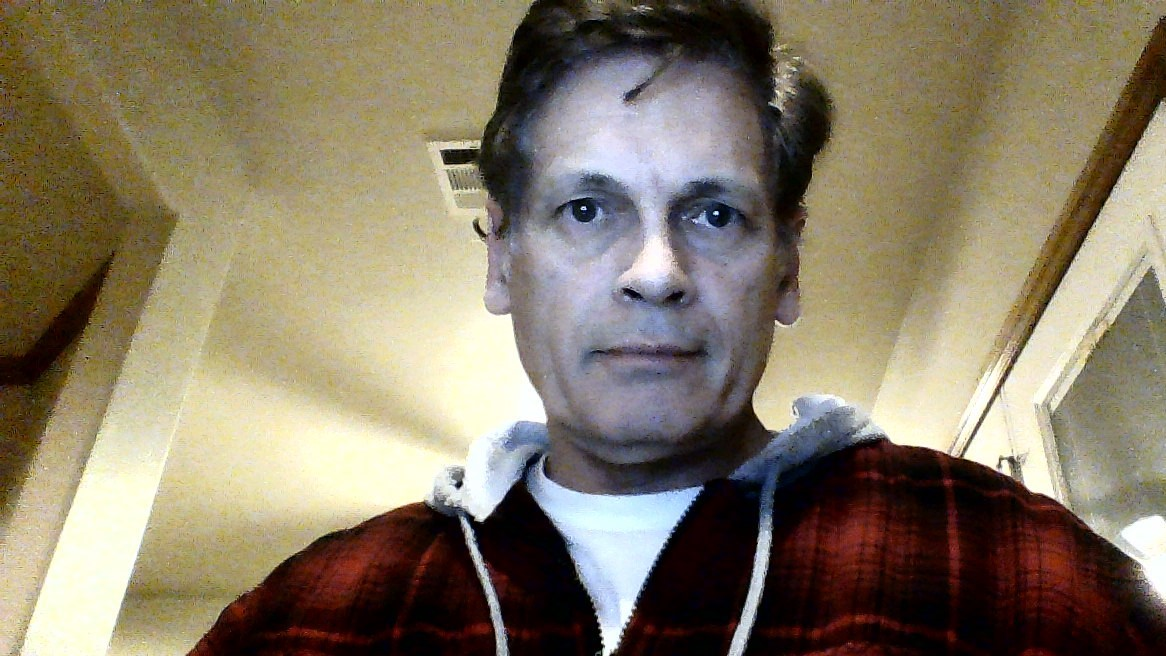
\includegraphics[width=0.20000\textwidth]{wayne.jpg}
\caption{Dr.~Wayne Stewart}
\end{figure}

\textless{}\center\textgreater{}

\section{Introduction}\label{introduction}

Here you should introduce the data and the problem you wish to solve.
Use your own subheadings. Fill with informative sentences and pictures
and links. You may inclucde sub-sub headings. You can cite from your
bibliography (see Millar 2011 and Crawley (2012))

\subsection{What are the variables?}\label{what-are-the-variables}

\begin{Shaded}
\begin{Highlighting}[]
\KeywordTok{data}\NormalTok{(mtcars)}
\KeywordTok{head}\NormalTok{(mtcars)}
\end{Highlighting}
\end{Shaded}

\begin{longtable}[]{@{}lrrrrrrrrrrr@{}}
\toprule
& mpg & cyl & disp & hp & drat & wt & qsec & vs & am & gear &
carb\tabularnewline
\midrule
\endhead
Mazda RX4 & 21.0 & 6 & 160 & 110 & 3.90 & 2.620 & 16.46 & 0 & 1 & 4 &
4\tabularnewline
Mazda RX4 Wag & 21.0 & 6 & 160 & 110 & 3.90 & 2.875 & 17.02 & 0 & 1 & 4
& 4\tabularnewline
Datsun 710 & 22.8 & 4 & 108 & 93 & 3.85 & 2.320 & 18.61 & 1 & 1 & 4 &
1\tabularnewline
Hornet 4 Drive & 21.4 & 6 & 258 & 110 & 3.08 & 3.215 & 19.44 & 1 & 0 & 3
& 1\tabularnewline
Hornet Sportabout & 18.7 & 8 & 360 & 175 & 3.15 & 3.440 & 17.02 & 0 & 0
& 3 & 2\tabularnewline
Valiant & 18.1 & 6 & 225 & 105 & 2.76 & 3.460 & 20.22 & 1 & 0 & 3 &
1\tabularnewline
\bottomrule
\end{longtable}

\begin{Shaded}
\begin{Highlighting}[]
\KeywordTok{names}\NormalTok{(mtcars)}
\end{Highlighting}
\end{Shaded}

\begin{verbatim}
##  [1] "mpg"  "cyl"  "disp" "hp"   "drat" "wt"   "qsec" "vs"   "am"   "gear"
## [11] "carb"
\end{verbatim}

\subsubsection{Sub sub headings can be
useful}\label{sub-sub-headings-can-be-useful}

\subsubsection{Plot data}\label{plot-data}

\begin{Shaded}
\begin{Highlighting}[]
\KeywordTok{library}\NormalTok{(ggplot2)}
\end{Highlighting}
\end{Shaded}

\begin{verbatim}
## Warning: package 'ggplot2' was built under R version 3.4.4
\end{verbatim}

\begin{Shaded}
\begin{Highlighting}[]
\NormalTok{g =}\StringTok{ }\KeywordTok{ggplot}\NormalTok{(mtcars, }\KeywordTok{aes}\NormalTok{(}\DataTypeTok{x =}\NormalTok{ disp, }\DataTypeTok{y =}\NormalTok{ mpg, }\DataTypeTok{color =}\NormalTok{ cyl)) }\OperatorTok{+}\StringTok{ }\KeywordTok{geom_point}\NormalTok{()}
\NormalTok{g =}\StringTok{ }\NormalTok{g }\OperatorTok{+}\StringTok{ }\KeywordTok{geom_smooth}\NormalTok{(}\DataTypeTok{method =} \StringTok{"loess"}\NormalTok{)}
\NormalTok{g}
\end{Highlighting}
\end{Shaded}

\begin{figure}
\centering
\includegraphics{project_files/figure-latex/carcharacteristics-1.pdf}
\caption{MTCARS}
\end{figure}

\subsection{How were the data
collected?}\label{how-were-the-data-collected}

\subsection{What is the story behind the
data?}\label{what-is-the-story-behind-the-data}

\subsection{Why was it gathered?}\label{why-was-it-gathered}

\subsection{What is your interest in the
data?}\label{what-is-your-interest-in-the-data}

\subsubsection{\texorpdfstring{Include pictures
\texttt{!{[}{]}(jpeg)}}{Include pictures !{[}{]}(jpeg)}}\label{include-pictures-jpeg}

\subsection{What problem do you wish to
solve?}\label{what-problem-do-you-wish-to-solve}

\section{Theory needed to carry out
SLR}\label{theory-needed-to-carry-out-slr}

\subsection{Main result 1}\label{main-result-1}

\subsection{Main result 2}\label{main-result-2}

\subsection{Main result 3 etc}\label{main-result-3-etc}

\section{Validity with mathematical
expressions}\label{validity-with-mathematical-expressions}

The following function was taken from
\url{https://rpubs.com/therimalaya/43190}

\subsection{Checks on validity}\label{checks-on-validity}

\subsubsection{Straight trend line}\label{straight-trend-line}

\paragraph{Use trendscatter}\label{use-trendscatter}

\subsubsection{Errors distributed
Normally}\label{errors-distributed-normally}

\[\epsilon_i \sim N(0,\sigma^2)\]

\paragraph{Shapiro-wilk}\label{shapiro-wilk}

\subsubsection{Constant variance}\label{constant-variance}

\paragraph{Residual vs fitted values}\label{residual-vs-fitted-values}

\paragraph{trendscatter on Residual Vs
Fitted}\label{trendscatter-on-residual-vs-fitted}

\subsubsection{\texorpdfstring{Zero mean value of
\(\epsilon\)}{Zero mean value of \textbackslash{}epsilon}}\label{zero-mean-value-of-epsilon}

\subsubsection{Independence of data}\label{independence-of-data}

\section{Analysis of the data}\label{analysis-of-the-data}

\subsection{Make sure you include many great
plots}\label{make-sure-you-include-many-great-plots}

\subsection{Add the trend to the data}\label{add-the-trend-to-the-data}

\subsection{Summary lm object}\label{summary-lm-object}

\subsubsection{Interpretation of all
tests}\label{interpretation-of-all-tests}

\subsubsection{Interpretation of multiple R
squared}\label{interpretation-of-multiple-r-squared}

\subsubsection{Interpretation of all point
estimates}\label{interpretation-of-all-point-estimates}

\subsection{\texorpdfstring{Calculate cis for \(\beta\) parameter
estimates}{Calculate cis for \textbackslash{}beta parameter estimates}}\label{calculate-cis-for-beta-parameter-estimates}

\subsubsection{\texorpdfstring{Use of
\texttt{predict()}}{Use of predict()}}\label{use-of-predict}

\subsubsection{\texorpdfstring{Use of
\texttt{ciReg()}}{Use of ciReg()}}\label{use-of-cireg}

\subsubsection{Check on outliers using cooks
plots}\label{check-on-outliers-using-cooks-plots}

Remember to interpret this plot and all other plots

\section{Model selection if you compared
models}\label{model-selection-if-you-compared-models}

\subsection{\texorpdfstring{Use adjusted
\(R^2\)}{Use adjusted R\^{}2}}\label{use-adjusted-r2}

\[R_{adj}^2 =\]

\section{Conclusion}\label{conclusion}

\subsection{Answer your research
question}\label{answer-your-research-question}

\subsection{Suggest ways to improve model or
experiment}\label{suggest-ways-to-improve-model-or-experiment}

\section*{References}\label{references}
\addcontentsline{toc}{section}{References}

\hypertarget{refs}{}
\hypertarget{ref-crawley}{}
Crawley, Michael J. 2012. ``Regression.'' In \emph{The R Book}, 449--97.
Chichester, UK: John Wiley \& Sons, Ltd.

\hypertarget{ref-millar}{}
Millar, Russell B. 2011. ``Latent Variable Models.'' In \emph{Statistics
in Practice}, 202--32. Chichester, UK: John Wiley \& Sons, Ltd.


\end{document}
